\documentclass[a4paper]{article}

\usepackage[utf8]{inputenc}
\usepackage[margin=1in]{geometry}
\usepackage[bookmarks]{hyperref}
\usepackage{graphicx}
\usepackage{listings}
\usepackage{color}
\usepackage{pdfpages}
\usepackage[style=verbose]{biblatex}
\usepackage{filecontents}

\def \IPF {\texttt{IPv4}}
\def \IPS {\texttt{IPv6}}
\hypersetup{
  pdfinfo={ee
    Title={COMP2207 IPv4/IPv6 Performance Report},
    Author={Huw Jones},
  },
  colorlinks=false,
  pdfborder=0 0 0,
}

\begin{filecontents}{bib.bib}
@online{ip_location,
  title = {IP Location Finder - Geolocation},
  url = {https://iplocation.net}
}
\end{filecontents}
\addbibresource{bib.bib}
\pagestyle{headings}

\author{Huw Jones\\27618153\\hcbj1g15}
\title{COMP2207 IPv4/IPv6 Performance Report}

\begin{document}
\maketitle
\newpage

\section{Data Gathering}
To gather the data, I decided to create a bash script.
The idea was to use the native \texttt{ping} and \texttt{ping6} commands available in standard POSIX compatible environments to do the actual pinging,
and then use the standard utilities to save the min/max/average/standard deviation data into a CSV file (along with the time and IP that was actually pinged).

My script had options to specify the number of pings and interval between pings.
I used bash's inbuilt \texttt{getopts} using flags in order to set these values.
I defaulted to setting the number of pings to 30 and the interval to 0.5 seconds.
This meant each test would take a minimum of 15 seconds and therefore each running of the script would take on average 25 to 30 minutes.

My script logged the time of day, the IP address (resolved from the hostname) and then min/max/average/standard deviation.
It logged the data independently for each host.
This meant each host's IPv4 and IPv6 data was kept in different files and therefore kept separate.
I chose to log this much data as it would give greater flexibility later when analysing the results.

I left my data gathering script running for about a day on two servers.
The first was the UG Login server (\texttt{uglogin.ecs.soton.ac.uk}: \texttt{152.78.71.152}, \texttt{2001:630:d0:f110:250:56ff:fea0:7d2}) which supports \IPF/\IPS.
The second is my own website/droplet (\texttt{huwcbjones.co.uk}: \texttt{46.101.18.128}, \texttt{2a03:b0c0:1:d0::9b:e001}) which also supports \IPF/\IPS.

I then wrote another quick bash script to extract the hostname, and average the average ping time.
This left me with a \texttt{summary.4.csv} file and a \texttt{summary.6.csv} file containing each host and the average ping from both servers.
I then combined these four files together along with the \texttt{Top100Sites.csv} in excel to produce a table of: rank, hostname, {\IPF} ping and {\IPS} ping.

As a small majority of the internet is accessible via \IPS, my script had to cater for not obtaining data for these sites.
I didn't actively add any code to handle this, but by chance my code enters a blank entry for that site.
This means you end up with blanks when a site was not accessible from \IPS.

\section{Results}
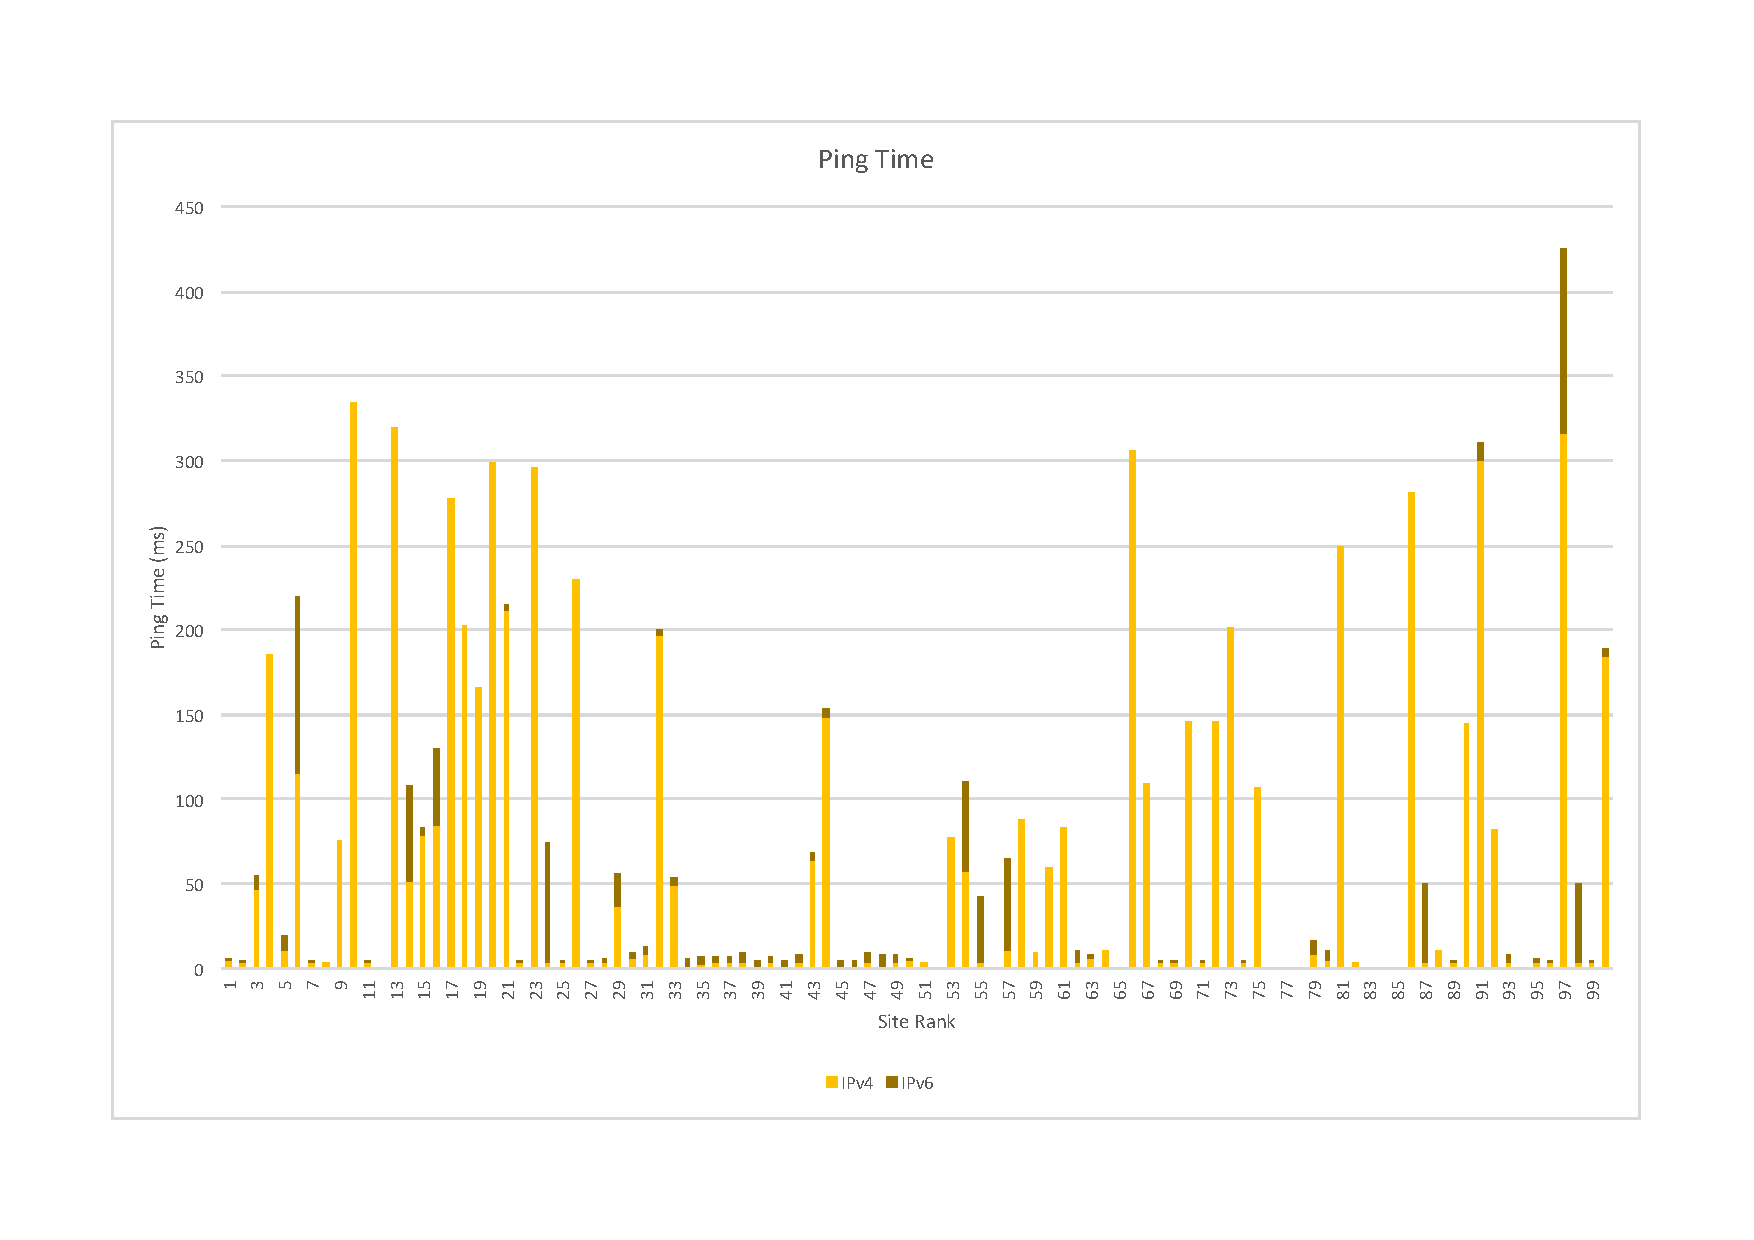
\includepdf[landscape=false,scale=0.9,angle=90,pagecommand={\subsection{Ping Time Stacked}}]{charts/stacked.pdf}
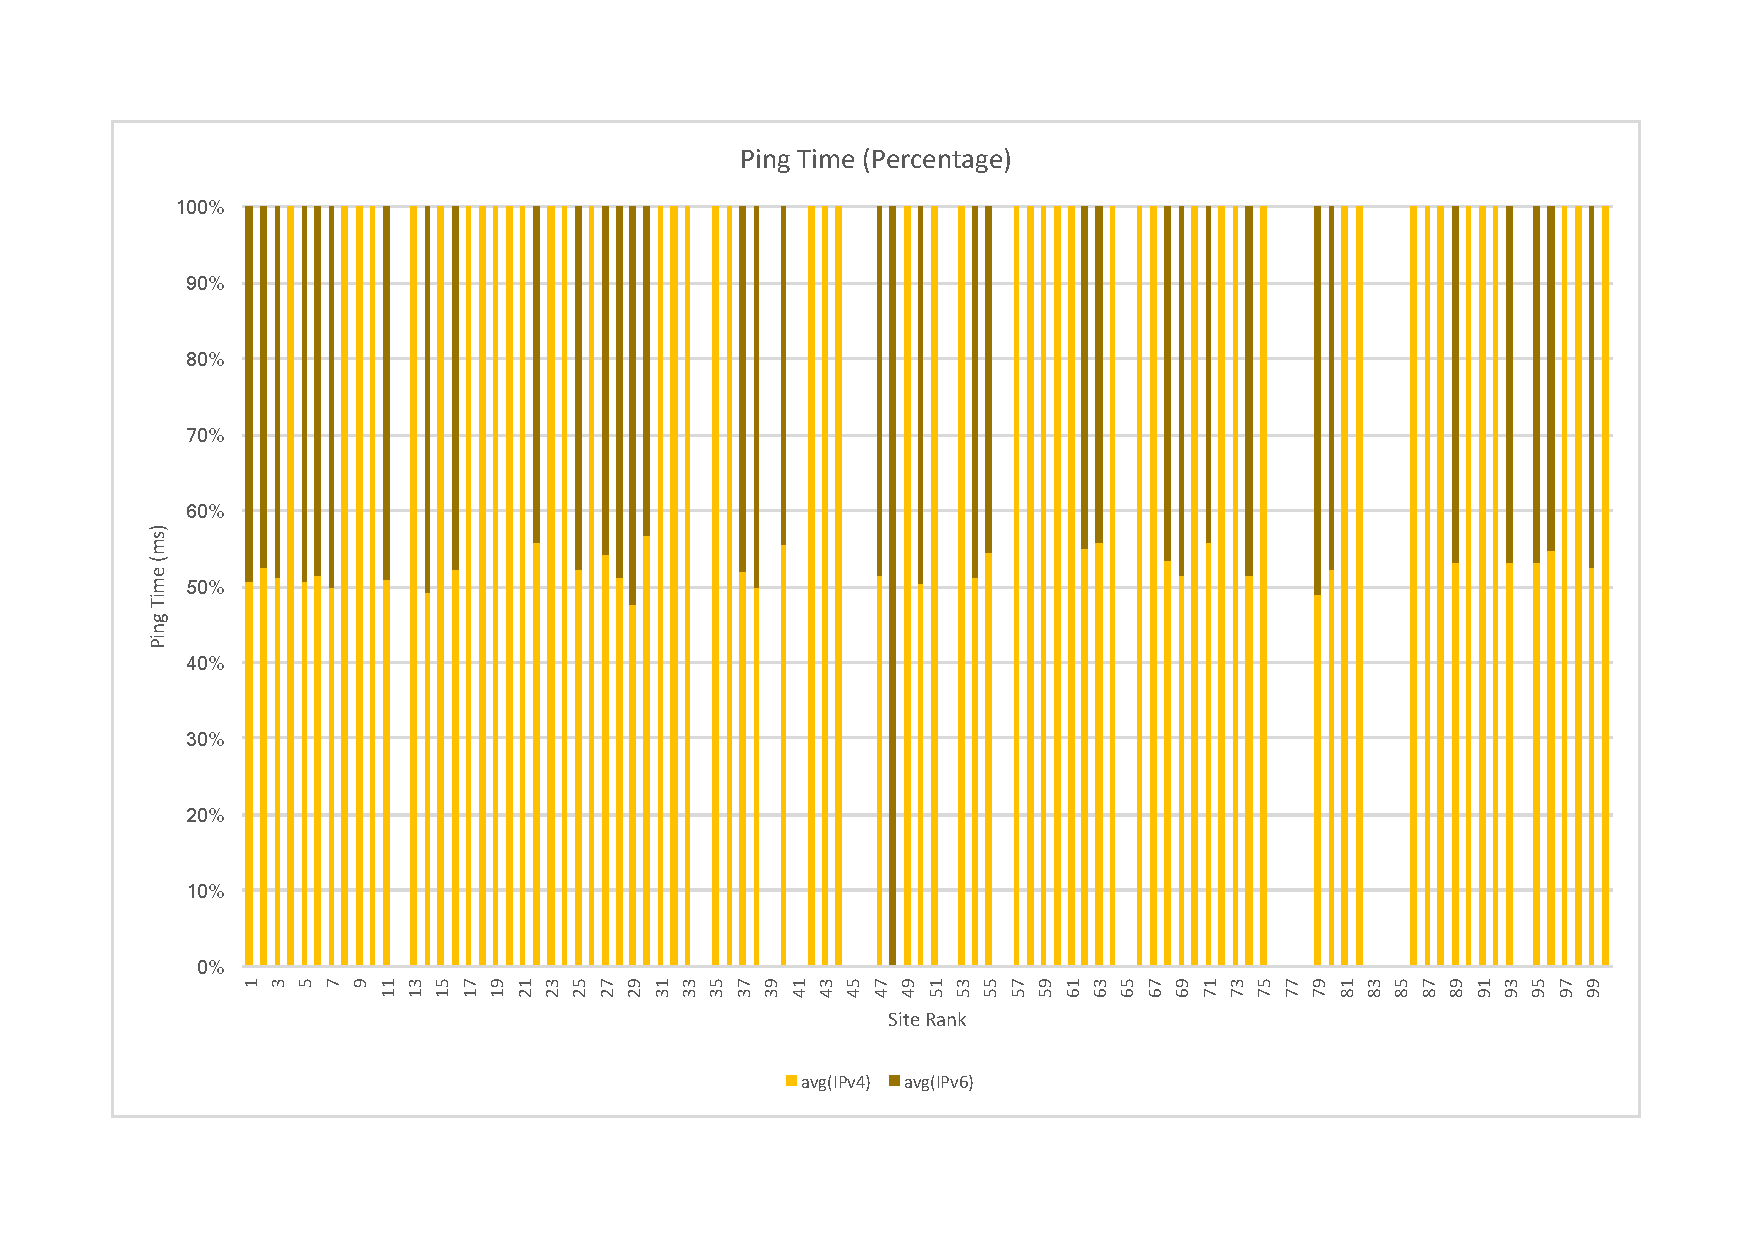
\includepdf[landscape=false,scale=0.9,angle=90,pagecommand={\subsection{Ping Time Stacked (Percentage)}}]{charts/stacked_percentage.pdf}

\section{Discussion}
Overall, there is no trend in {\IPF}/{\IPS} ping times down the top 100 list.
This is most probably due to the fact that different sites are popular in different countries.

Even though \texttt{baidu.com} is the $4^\textrm{th}$ most popular site, it's ping put it $68^\textrm{th}$ out of the top 100.
All the IP addresses pinged (\texttt{111.13.101.208}, \texttt{123.125.114.144}, \texttt{180.149.132.47} \& \texttt{220.181.57.217})
  indicate that their servers are hosted in China.\footcite{ip_location}
This means it is physically impossible to be quick.

\newpage
\printbibliography
\end{document}
